This section demonstrates the practical application of the extension through two common developer workflows: analyzing a single commit and comparing two different commits.

\subsection{Use Case 1: Analyzing a Single Commit}
A common task for a developer is to understand the changes introduced in a specific commit. This might be during a code review or when debugging a feature.

\begin{enumerate}
    \item \textbf{Action}: The user opens the Git Graph view and clicks on a commit in the graph.
    \item \textbf{Immediate Response}: The Commit Details view opens instantly, showing the commit author, message, and a list of changed files. A loading animation is displayed in the "AI Analysis" section (as shown in Figure \ref{fig:use-case-1-loading}).
    \item \textbf{Asynchronous Update}: After a few seconds, the AI analysis result is pushed to the UI, replacing the loading indicator with a concise, structured summary of the commit's purpose, impact, and quality (see Figure \ref{fig:use-case-1-loaded}).
\end{enumerate}

\begin{figure}[h!]
    \centering
    % TODO: Add a screenshot of the commit details view right after clicking,
    % showing the AI analysis section with a loading spinner/message.
    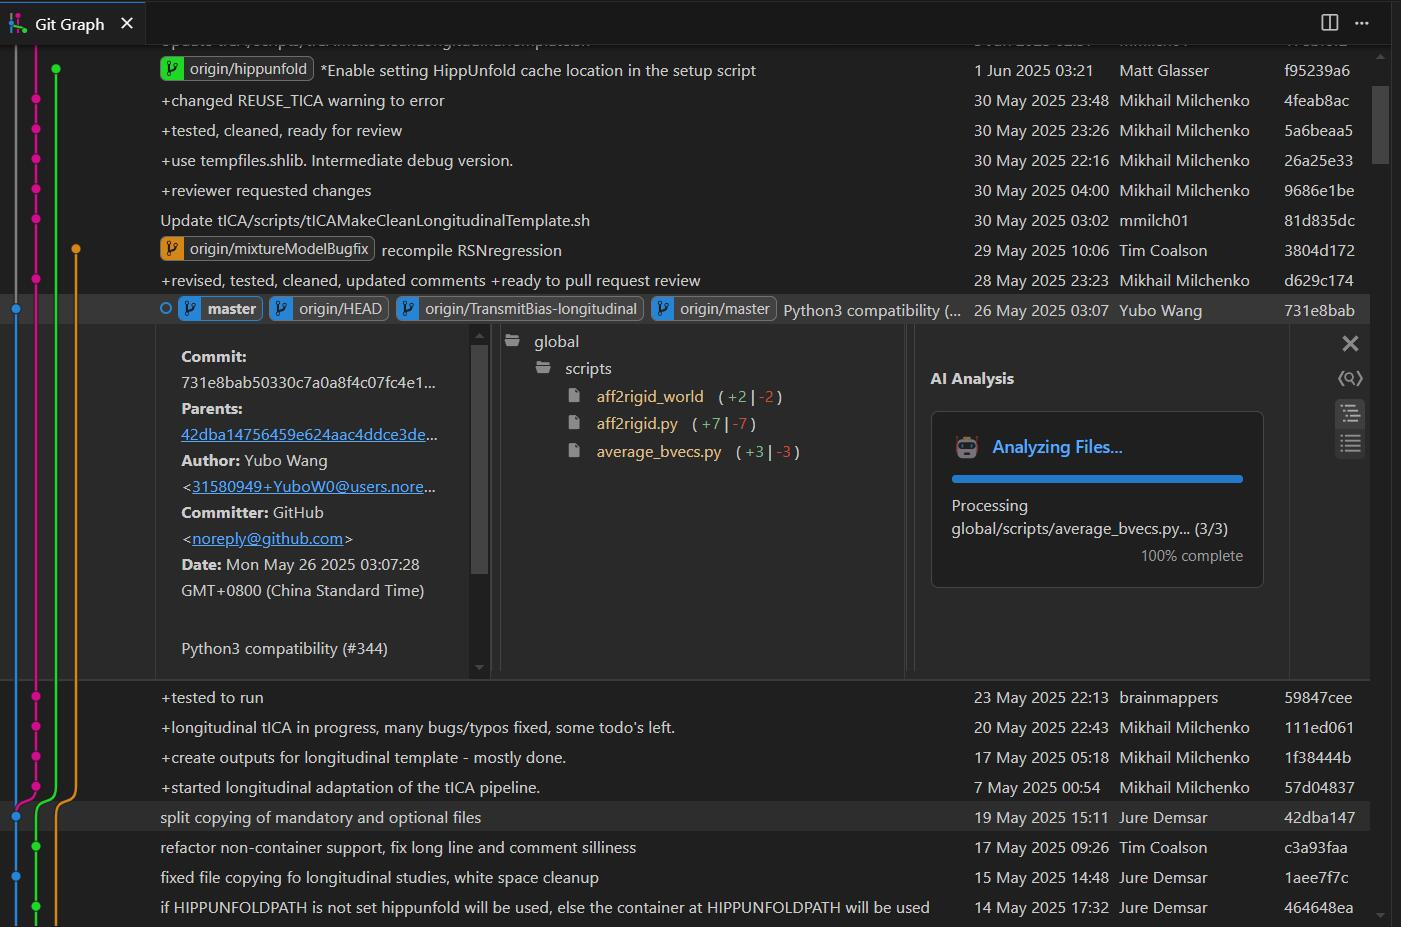
\includegraphics[width=0.9\textwidth]{figures/use-case-1-loading.jpg}
    \caption{The Commit Details view immediately after selection, with the AI Analysis section in a loading state.}
    \label{fig:use-case-1-loading}
\end{figure}

\begin{figure}[h!]
    \centering
    % TODO: Add a screenshot of the same view after the AI analysis has loaded,
    % showing the generated summary.
    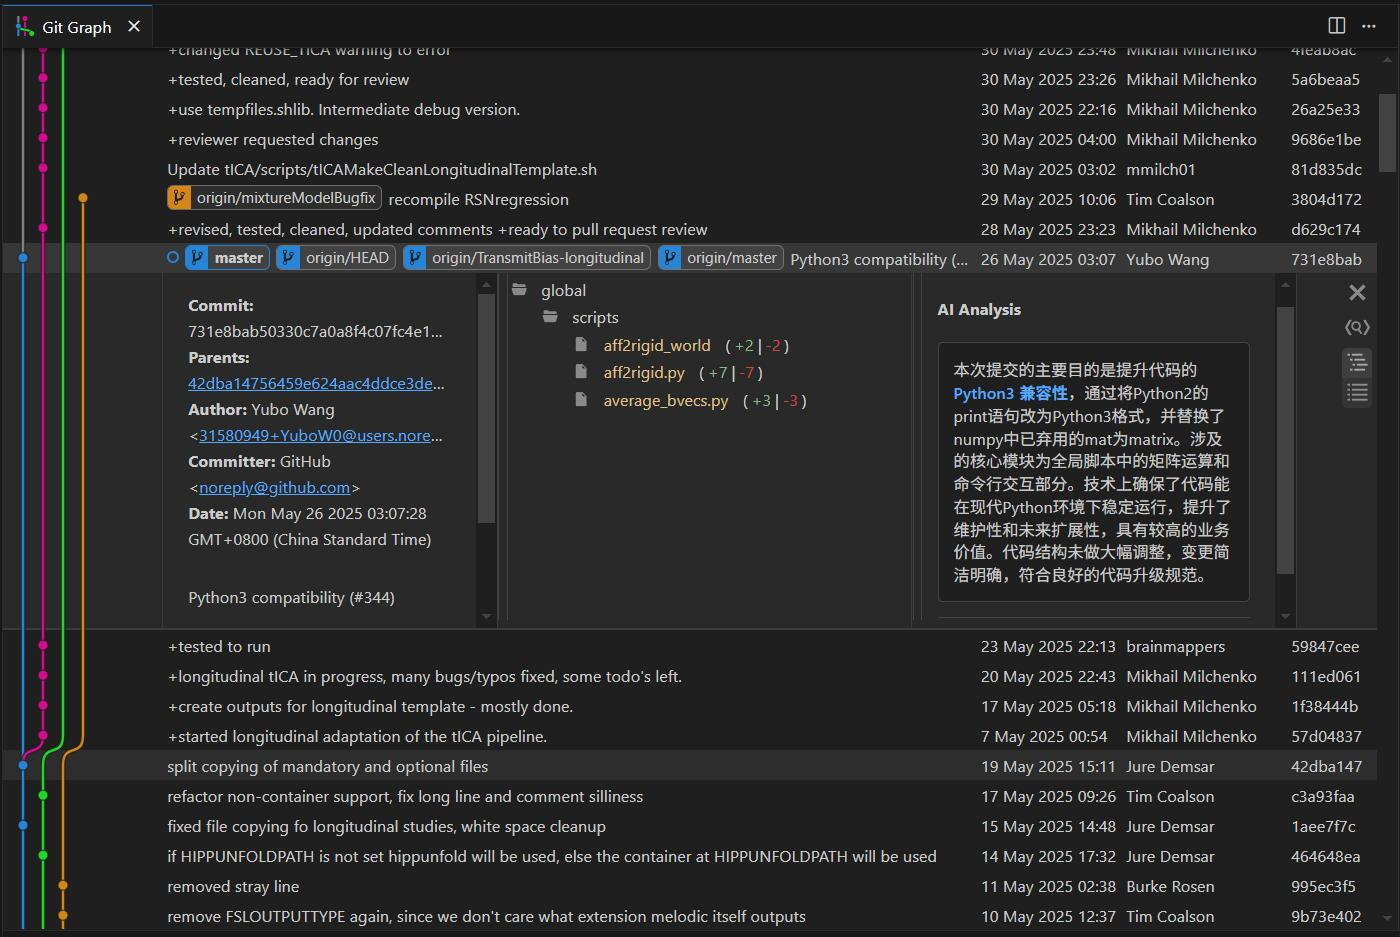
\includegraphics[width=0.9\textwidth]{figures/use-case-1-loaded.jpg}
    \caption{The AI-generated summary is asynchronously loaded and displayed, providing a high-level overview of the changes.}
    \label{fig:use-case-1-loaded}
\end{figure}


\subsection{Use Case 2: Comparing Two Commits}
Another powerful feature is the ability to understand the cumulative changes between any two points in the repository's history, such as comparing a feature branch head against the main branch.

\begin{enumerate}
    \item \textbf{Action}: The user clicks on a commit, then holds CTRL/CMD and clicks on a second commit.
    \item \textbf{Response}: The view immediately lists all files that were changed between these two commits. The AI analysis section shows a loading state.
    \item \textbf{Result}: The AI-generated summary appears, focusing on the high-level evolution between the two versions, highlighting major feature changes or refactoring efforts (as depicted in Figure \ref{fig:use-case-2-comparison}).
\end{enumerate}

\begin{figure}[h!]
    \centering
    % TODO: Add a screenshot of the comparison view, showing the list of changed
    % files and the AI-generated summary of the changes between the two commits.
    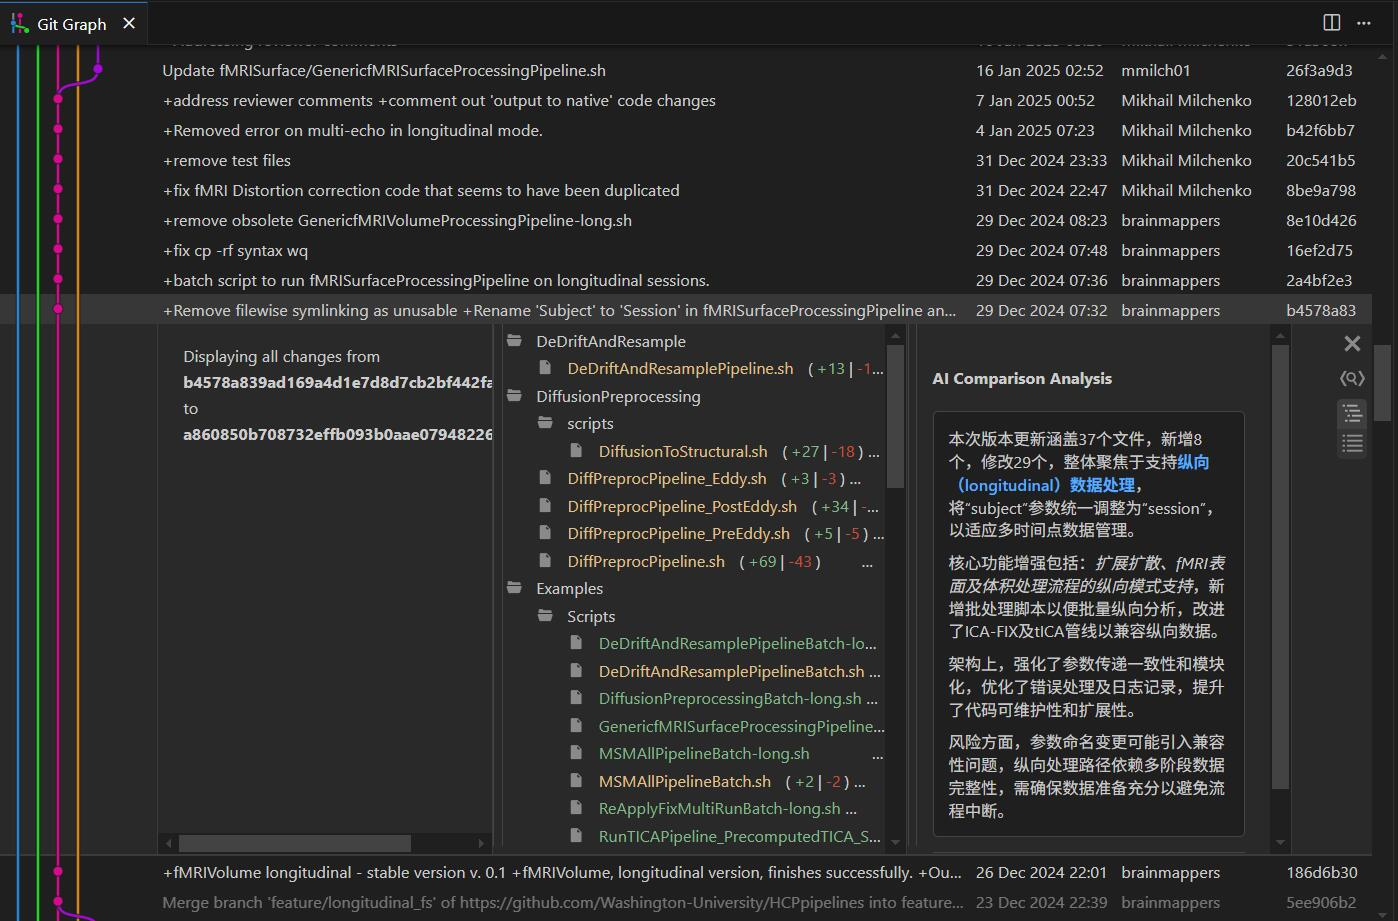
\includegraphics[width=0.9\textwidth]{figures/use-case-2-comparison.jpg}
    \caption{AI analysis of the differences between two commits, summarizing the overall changes.}
    \label{fig:use-case-2-comparison}
\end{figure}

\subsection{Use Case 3: In-Depth File Evolution Analysis}
To understand the full lifecycle of a specific file, developers can use the dedicated File History view.

\begin{enumerate}
    \item \textbf{Action}: In the main Git Graph view, the user right-clicks on a file within the commit details and selects "View File History in New Tab".
    \item \textbf{Evolution Analysis}: A new VS Code tab opens instantly, displaying the file's commit history list and statistics. After a few seconds, the panel is populated with an AI-generated analysis of the file's entire evolution, including key changes and patterns (Figure \ref{fig:use-case-3-history-loaded}).
    \item \textbf{Version Comparison}: The user can then switch to the "Version Compare" tab, select any two commits from the list, and receive a targeted AI analysis comparing just those two versions (Figure \ref{fig:use-case-3-version-compare}).
\end{enumerate}


\begin{figure}[h!]
    \centering
    % TODO: Add a screenshot of the File History tab after the AI analysis is loaded.
    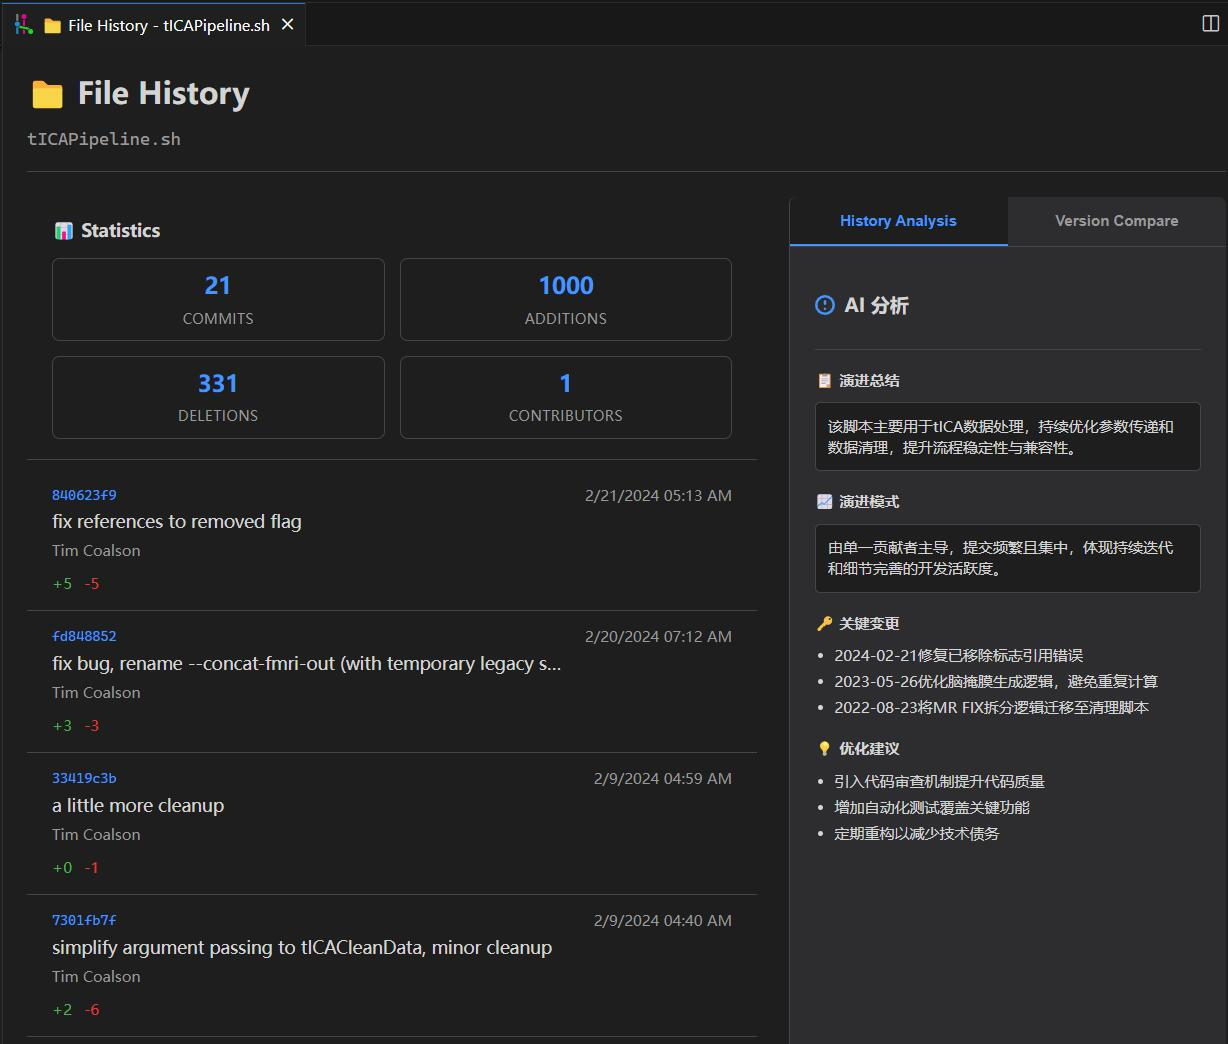
\includegraphics[width=0.9\textwidth]{figures/use-case-3-history-loaded.jpg}
    \caption{The AI analysis, showing the file's evolution summary and patterns.}
    \label{fig:use-case-3-history-loaded}
\end{figure}

\begin{figure}[h!]
    \centering
    % TODO: Add a screenshot of the "Version Compare" tab with two versions selected and compared.
    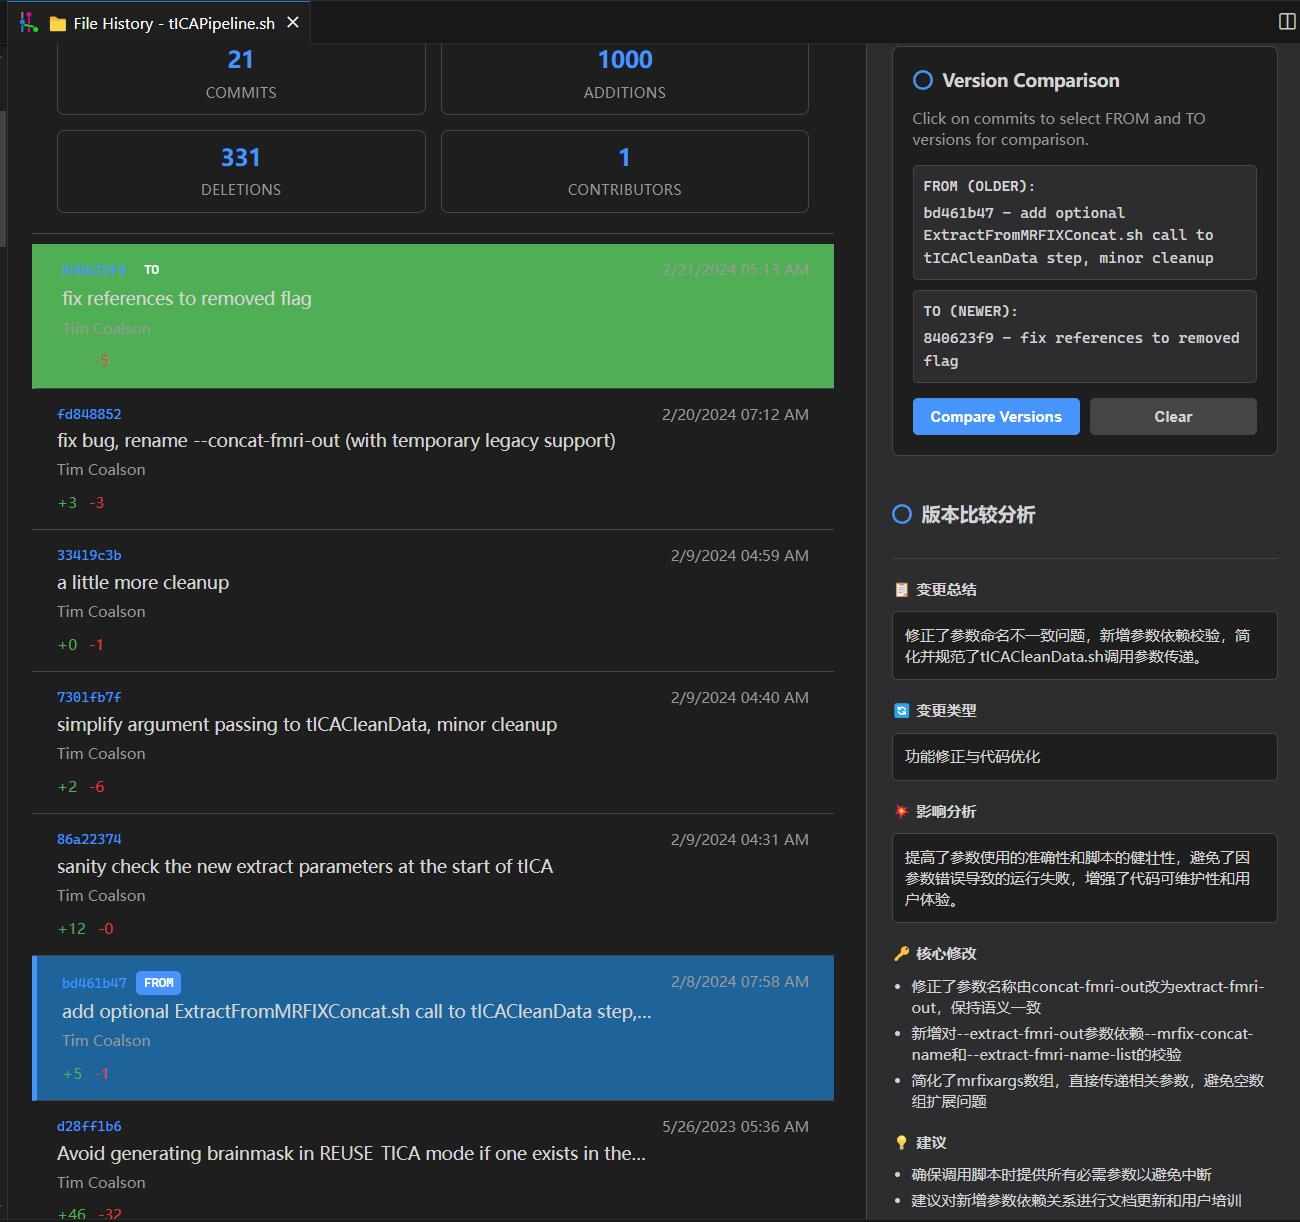
\includegraphics[width=0.9\textwidth]{figures/use-case-3-version-compare.jpg}
    \caption{The "Version Compare" mode, showing a targeted AI analysis between two selected commits for the file.}
    \label{fig:use-case-3-version-compare}
\end{figure} 